\documentclass{roadef}
\usepackage{amsmath}

% \usepackage{fontspec}
% This command is to use simple quotes inside math expressions:
\newcommand{\mq}[1] {#1\textrm'}

\begin{document}


% Le titre du papier
\title{ROADEF Challenge 2018: }

% Le titre court
% \def\shorttitle{Titre court}

\author{Franco Peschiera\inst{1}, Nicolas Dupin\inst{1}}


\institute{
ISAE-SUPAERO, Universit� de Toulouse, France \\
\email{\{franco.peschiera,nicolas.dupin\}@isae-supaero.fr}
}


\maketitle
\thispagestyle{empty}

% \keywords{optimization, planning, military, maintenance}


\section{Introduction}

\section{The problem}

    \subsection{Definitions}

        \begin{itemize}

            \item Tree: first node. Corresponds to a Jumbo. A node without a parent.
            \item Node: tree representation of an Item. It has a parent and can have children or be a Leaf.
            \item Forest: a list of Trees, corresponding to the solution for an instance or Batch.
            \item Solution: same as Forest. The result of an instance. Should comply with constraints.
            \item Child: a Node that is obtained by cutting a bigger node. All nodes are children of another node except the tree or first node.
            \item Leaf: a Node that has no children. Corresponds to an Item or to a Waste. Or to a residual.
            \item Swap: the act of taking two Nodes and switching their places, while taking into account the differences in space. The result needs to still keep the logic of the Jumbo / Tree structure.
            \item Insert: just like the Swap but only the first node is inserted just before the second node. The second node is not moved.
            \item Level: Nodes of level 1 are the nodes that have CUT parameter equal to 1. A level 1 swap is a swap between nodes of level 1.

        \end{itemize}

\section{Solution coding}

    \subsection{Data structures}

        The solution is stored as a forest.

    \subsection{Trees and nodes}

        If a node is not a leaf, then it has been cut. Its children represent the number of cuts it has received, following the rules of guillotine cuts.
        Each children node has a level that is 1 bigger than its parent. This way we can track the level a node is in (and the number of cuts we had to do to arrive to the node).

        For example, the solution shown in figure \ref{fig:case1} is represented by the following tree:

        \begin{verbatim}
                      /-2
                     |
                   /1|--3
                  |  |
                  |  |   /-5
                  |   \4|
                  |      \-6
                  |
                  |   /-8
                  |-7|
                  |   \-9
                -0|
                  |   /-11
                  |  |
                  |  |   /-13
                  |-10-12
                  |  |   \-14
                  |  |
                  |   \-15
                  |
                   \-16

        \end{verbatim}

        \begin{figure}
            \centering
            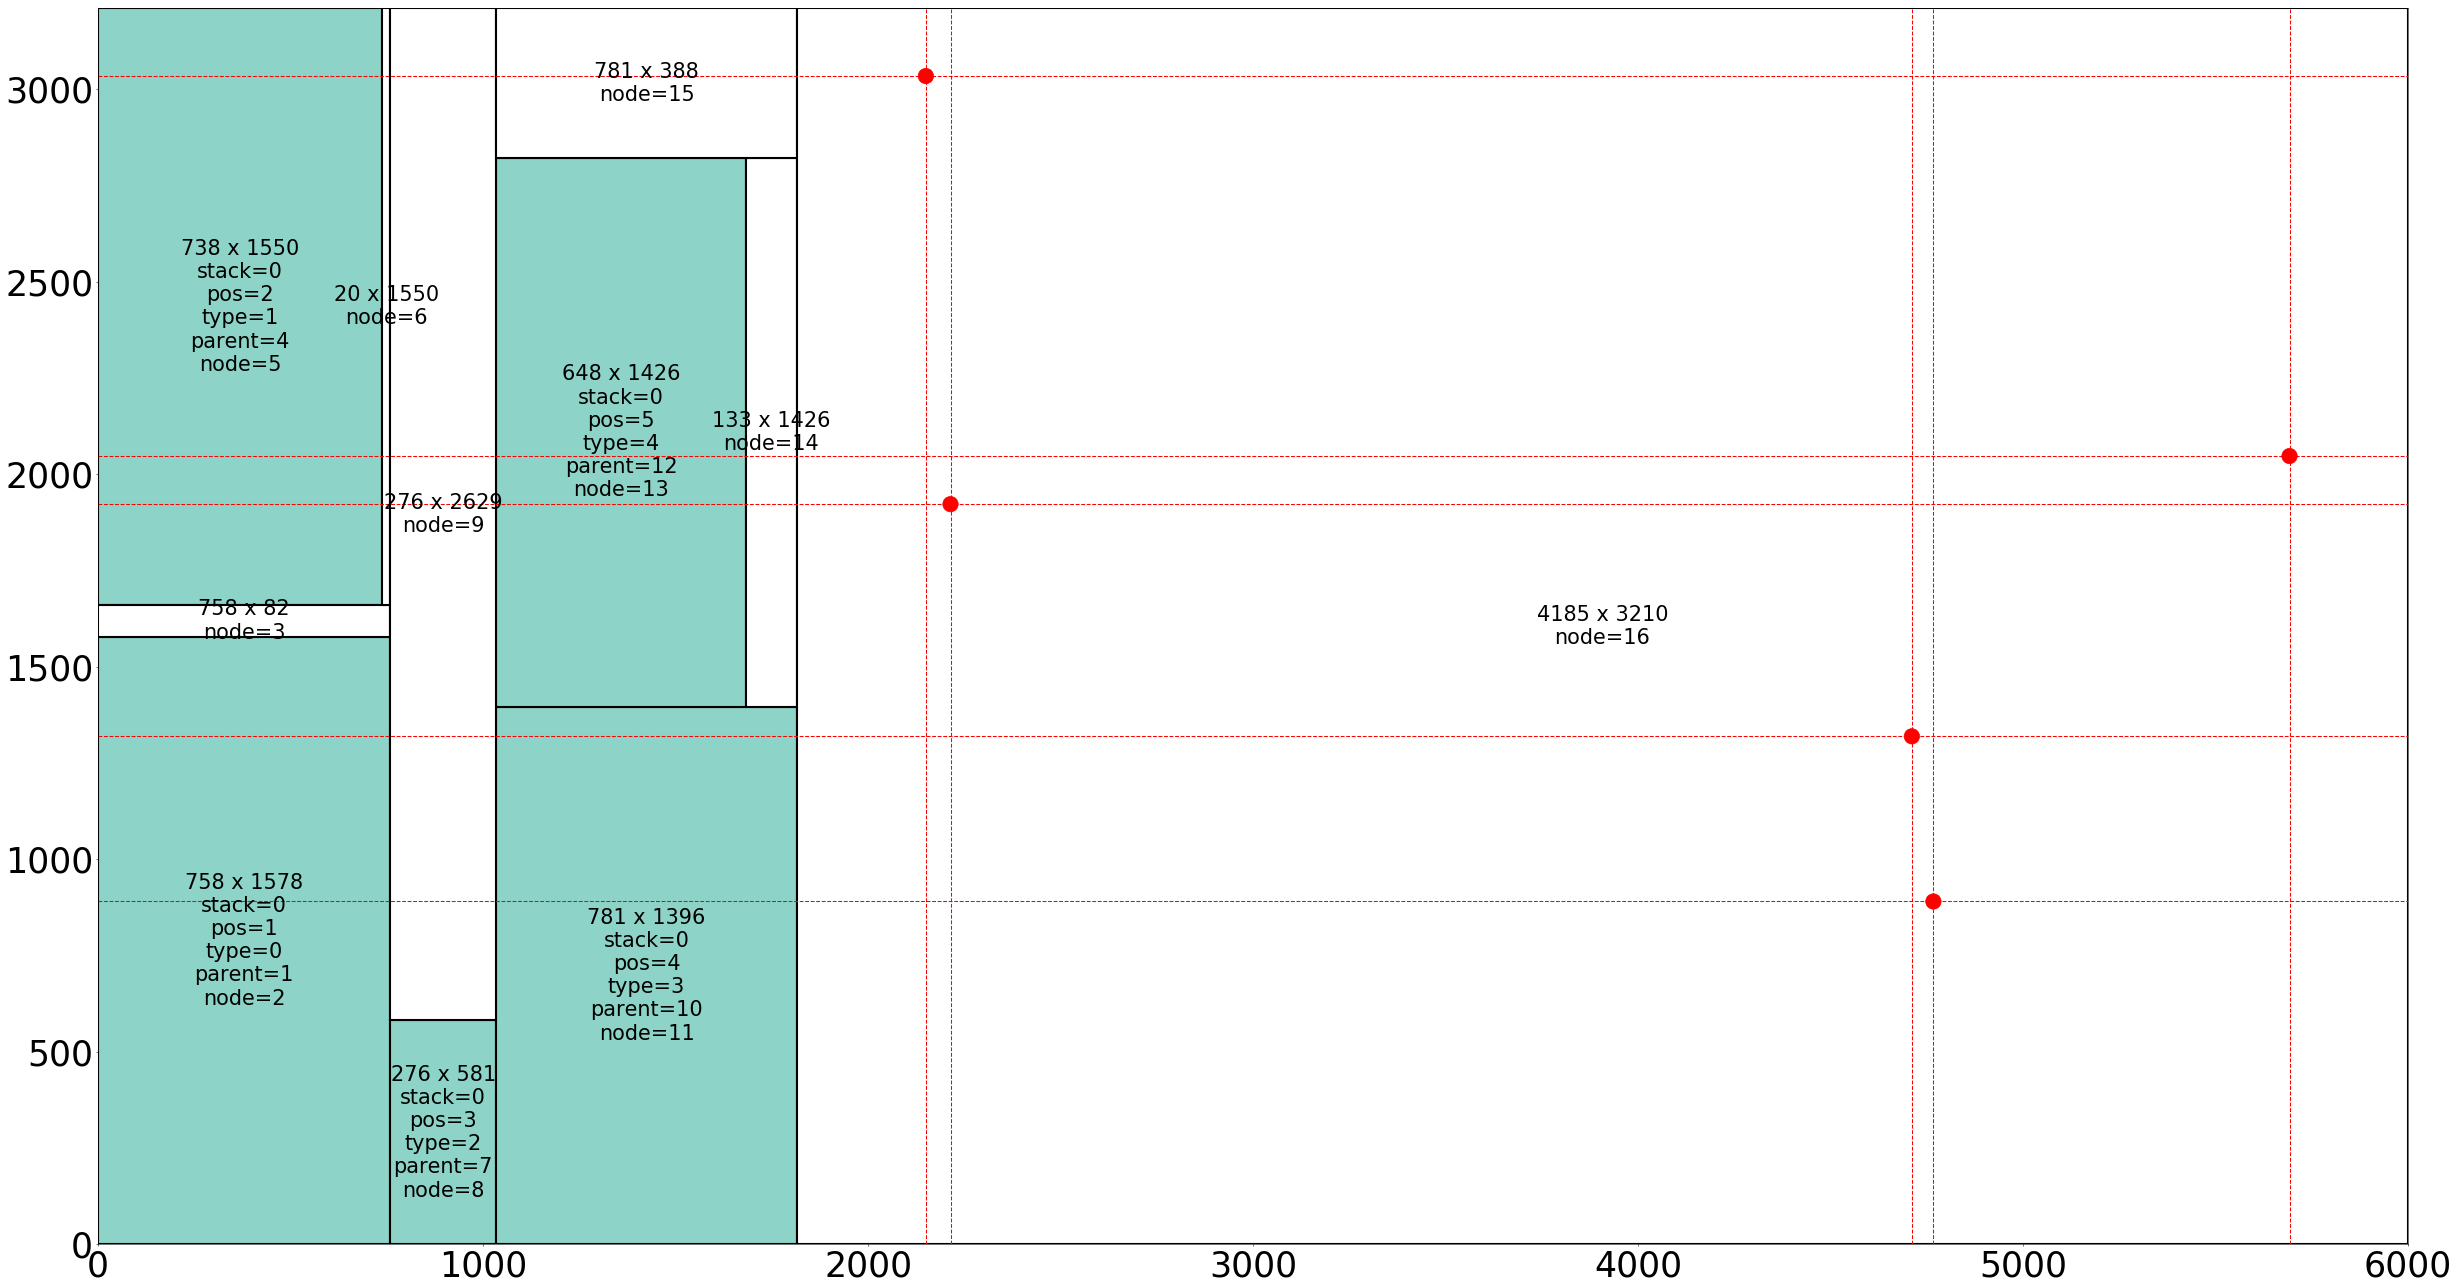
\includegraphics[width=0.7\linewidth]{case1_heur.png}
            \caption{case1 solution} \label{fig:case1}
        \end{figure}

        The information present in a node, besides the regular graph information, is:

        \begin{itemize}

            \item Size: WIDTH, HEIGHT
            \item Position: PLATE\_ID, X, Y
            \item CUT: the number of cuts needed to make to arrive to the node.
            \item TYPE: following the specified format: waste, intermediate node or an item.

        \end{itemize}

\section{Allowed moves}

    Swaps can be "real swaps" or just "an insertion". We call everything swaps even if they are just inserts.
    Also, they can include the rotation of none, the first, the second, or both nodes.
    Finally, the nodes can be in the same level or in different levels.

    \subsection{Checking swaps}

        In order to make a feasible swap, it's necessary to check the following:

        \begin{itemize}

            \item In a swap: each node is smaller than the space left by the other node plus the available waste.
            \item In an insert: the inserted node needs to be smaller than the available waste next to the other node.

        \end{itemize}

        If there's space, in theory we should be able to do it.

        To evaluate the improvement of the swap we need to:

        \begin{enumerate}

            \item Calculate the balance of sequence violations.
            \item Calculate the balance of defects violations.
            \item Calculate the balance of density of waste moved to the right.

        \end{enumerate}

        These three terms, weighted by some parameters, will determine if the swap is done. Here, there is always an element of randomness based on the temperature.

    \subsection{Inserting a node somewhere}

        This is the basic logic to insert a node inside a destination node. This is use as the base for all the swaps mentioned above.

        \begin{enumerate}

            \item Take out children waste from each node. This is the waste that's at the end if any.
            \item If only child, take out and decrease level.
            \item If rotation is needed, rotate the whole node.
            \item Insert node in its destination parent.
            \item If the level of the node has changed, update it.
            \item if the node corresponds to actually several nodes, get them out and re-insert them.
            \item if needed, add a children waste on the node(s) that has /have just been inserted.
            \item Since a node has just been inserted, modify the residual waste at the end of the destination node.

        \end{enumerate}

    \subsection{Regular insert}

        Figures \ref{fig:swap2-before} and \ref{fig:swap2-after} show an example of a level 2 insert.
        The node 110 (red) is inserted just before the node 107 (yellow). This is a move that is also beneficial because it takes wastes to the right.

        \begin{figure}
            \centering
            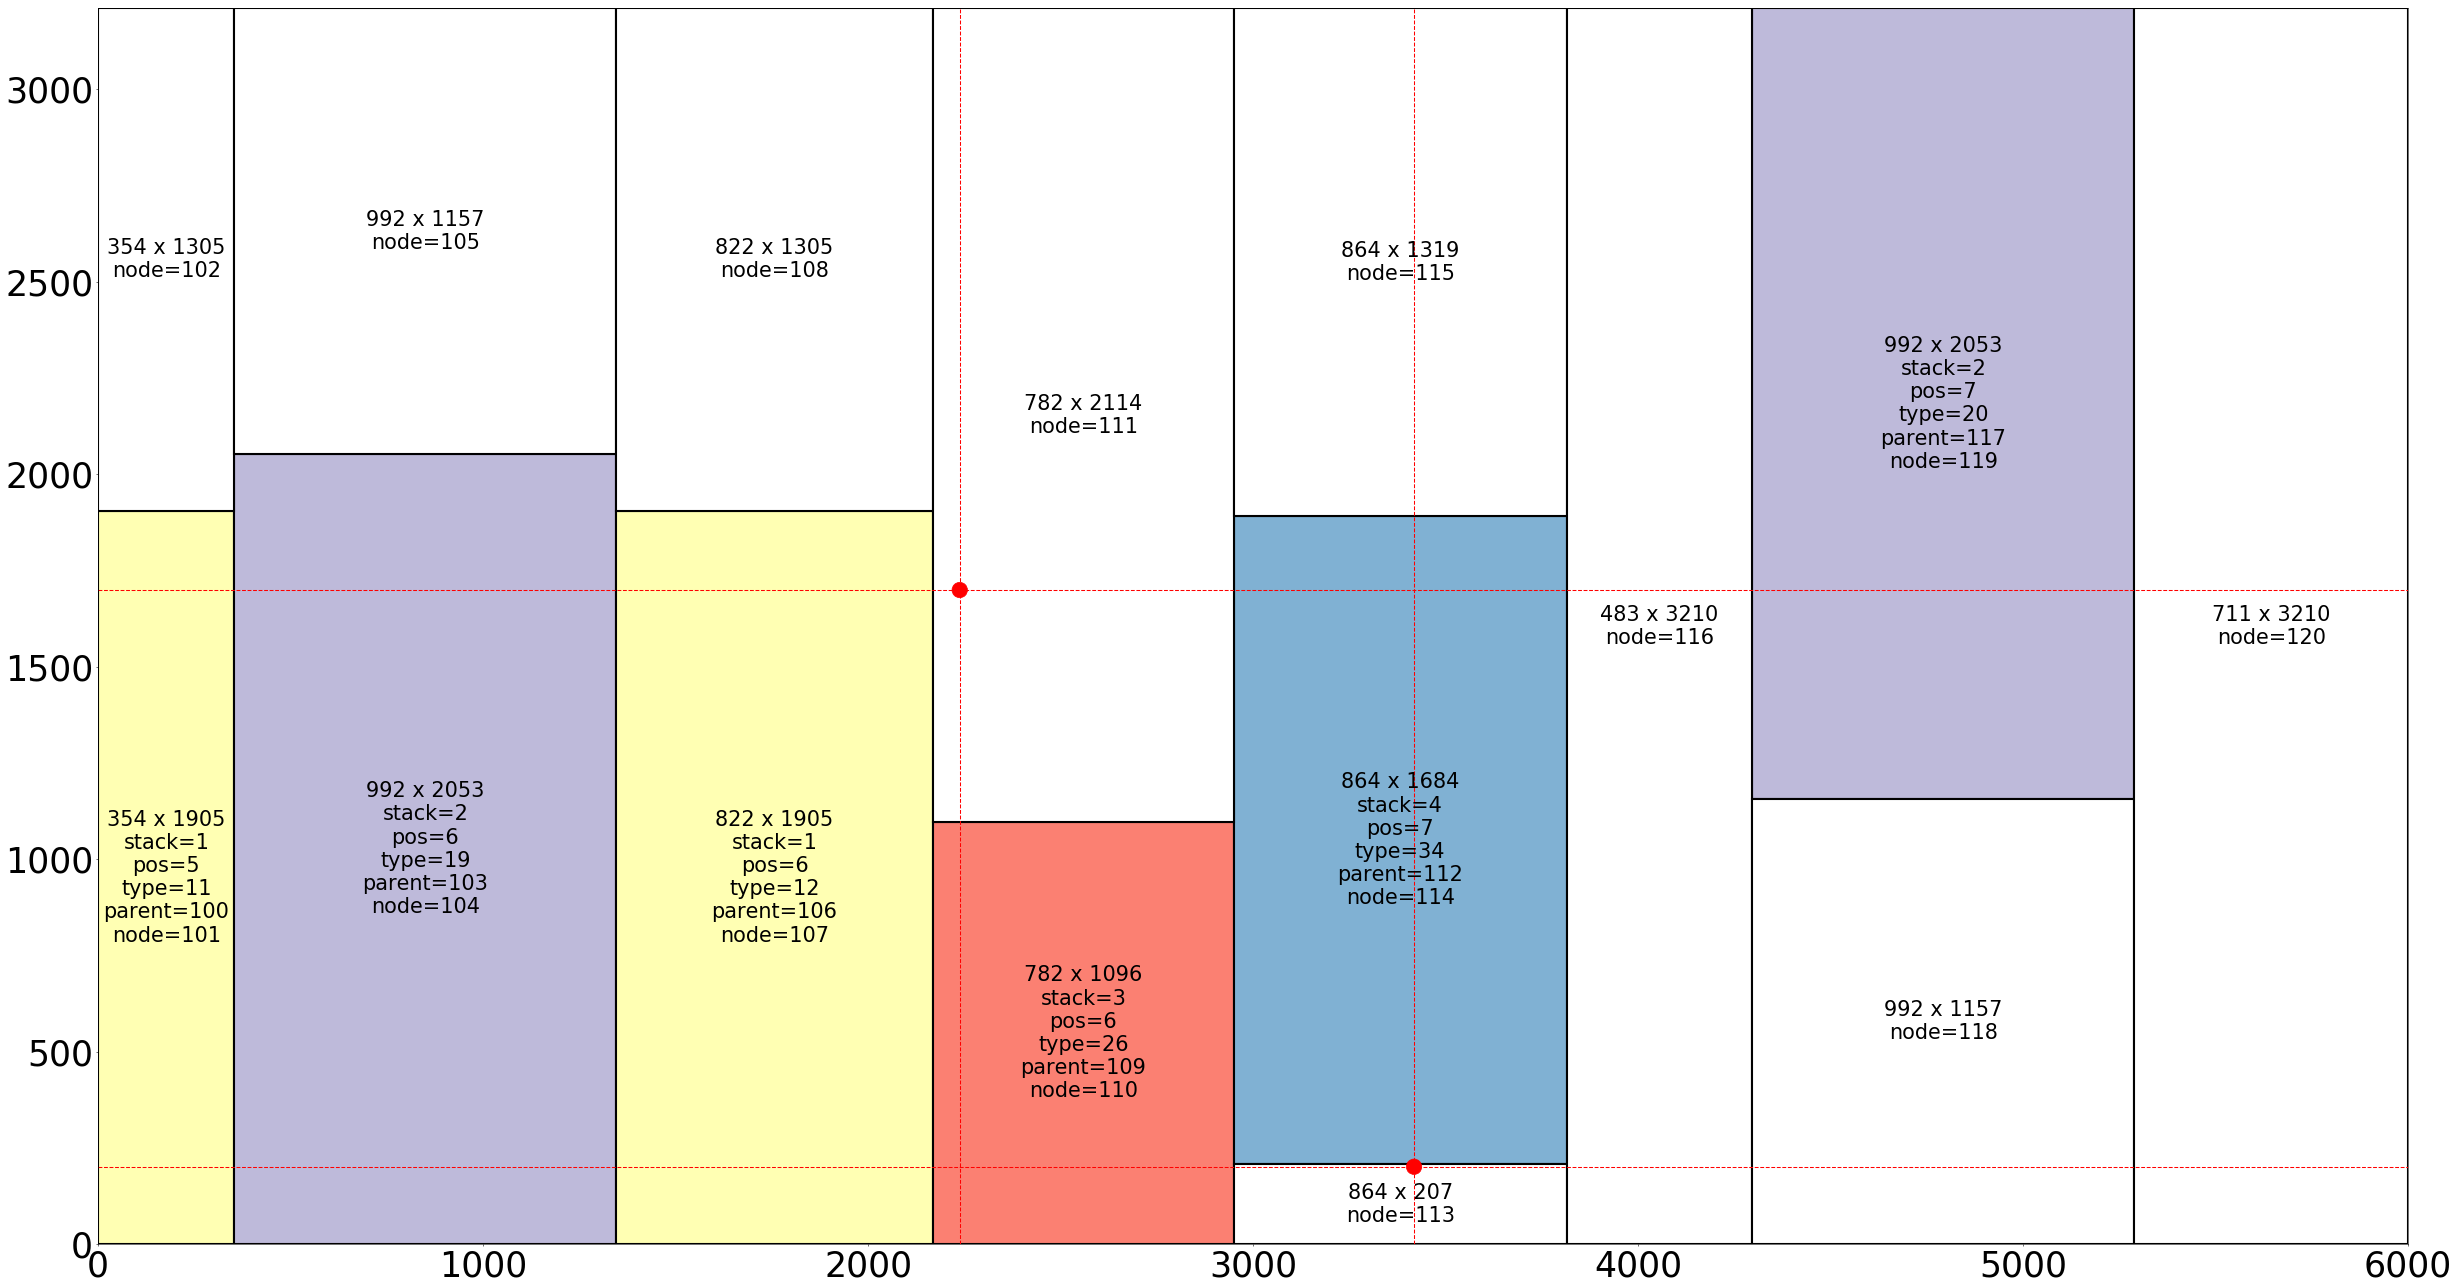
\includegraphics[width=0.7\linewidth]{swap_2_before.png}
            \caption{before swap level 2} \label{fig:swap2-before}
        \end{figure}

        \begin{figure}
            \centering
            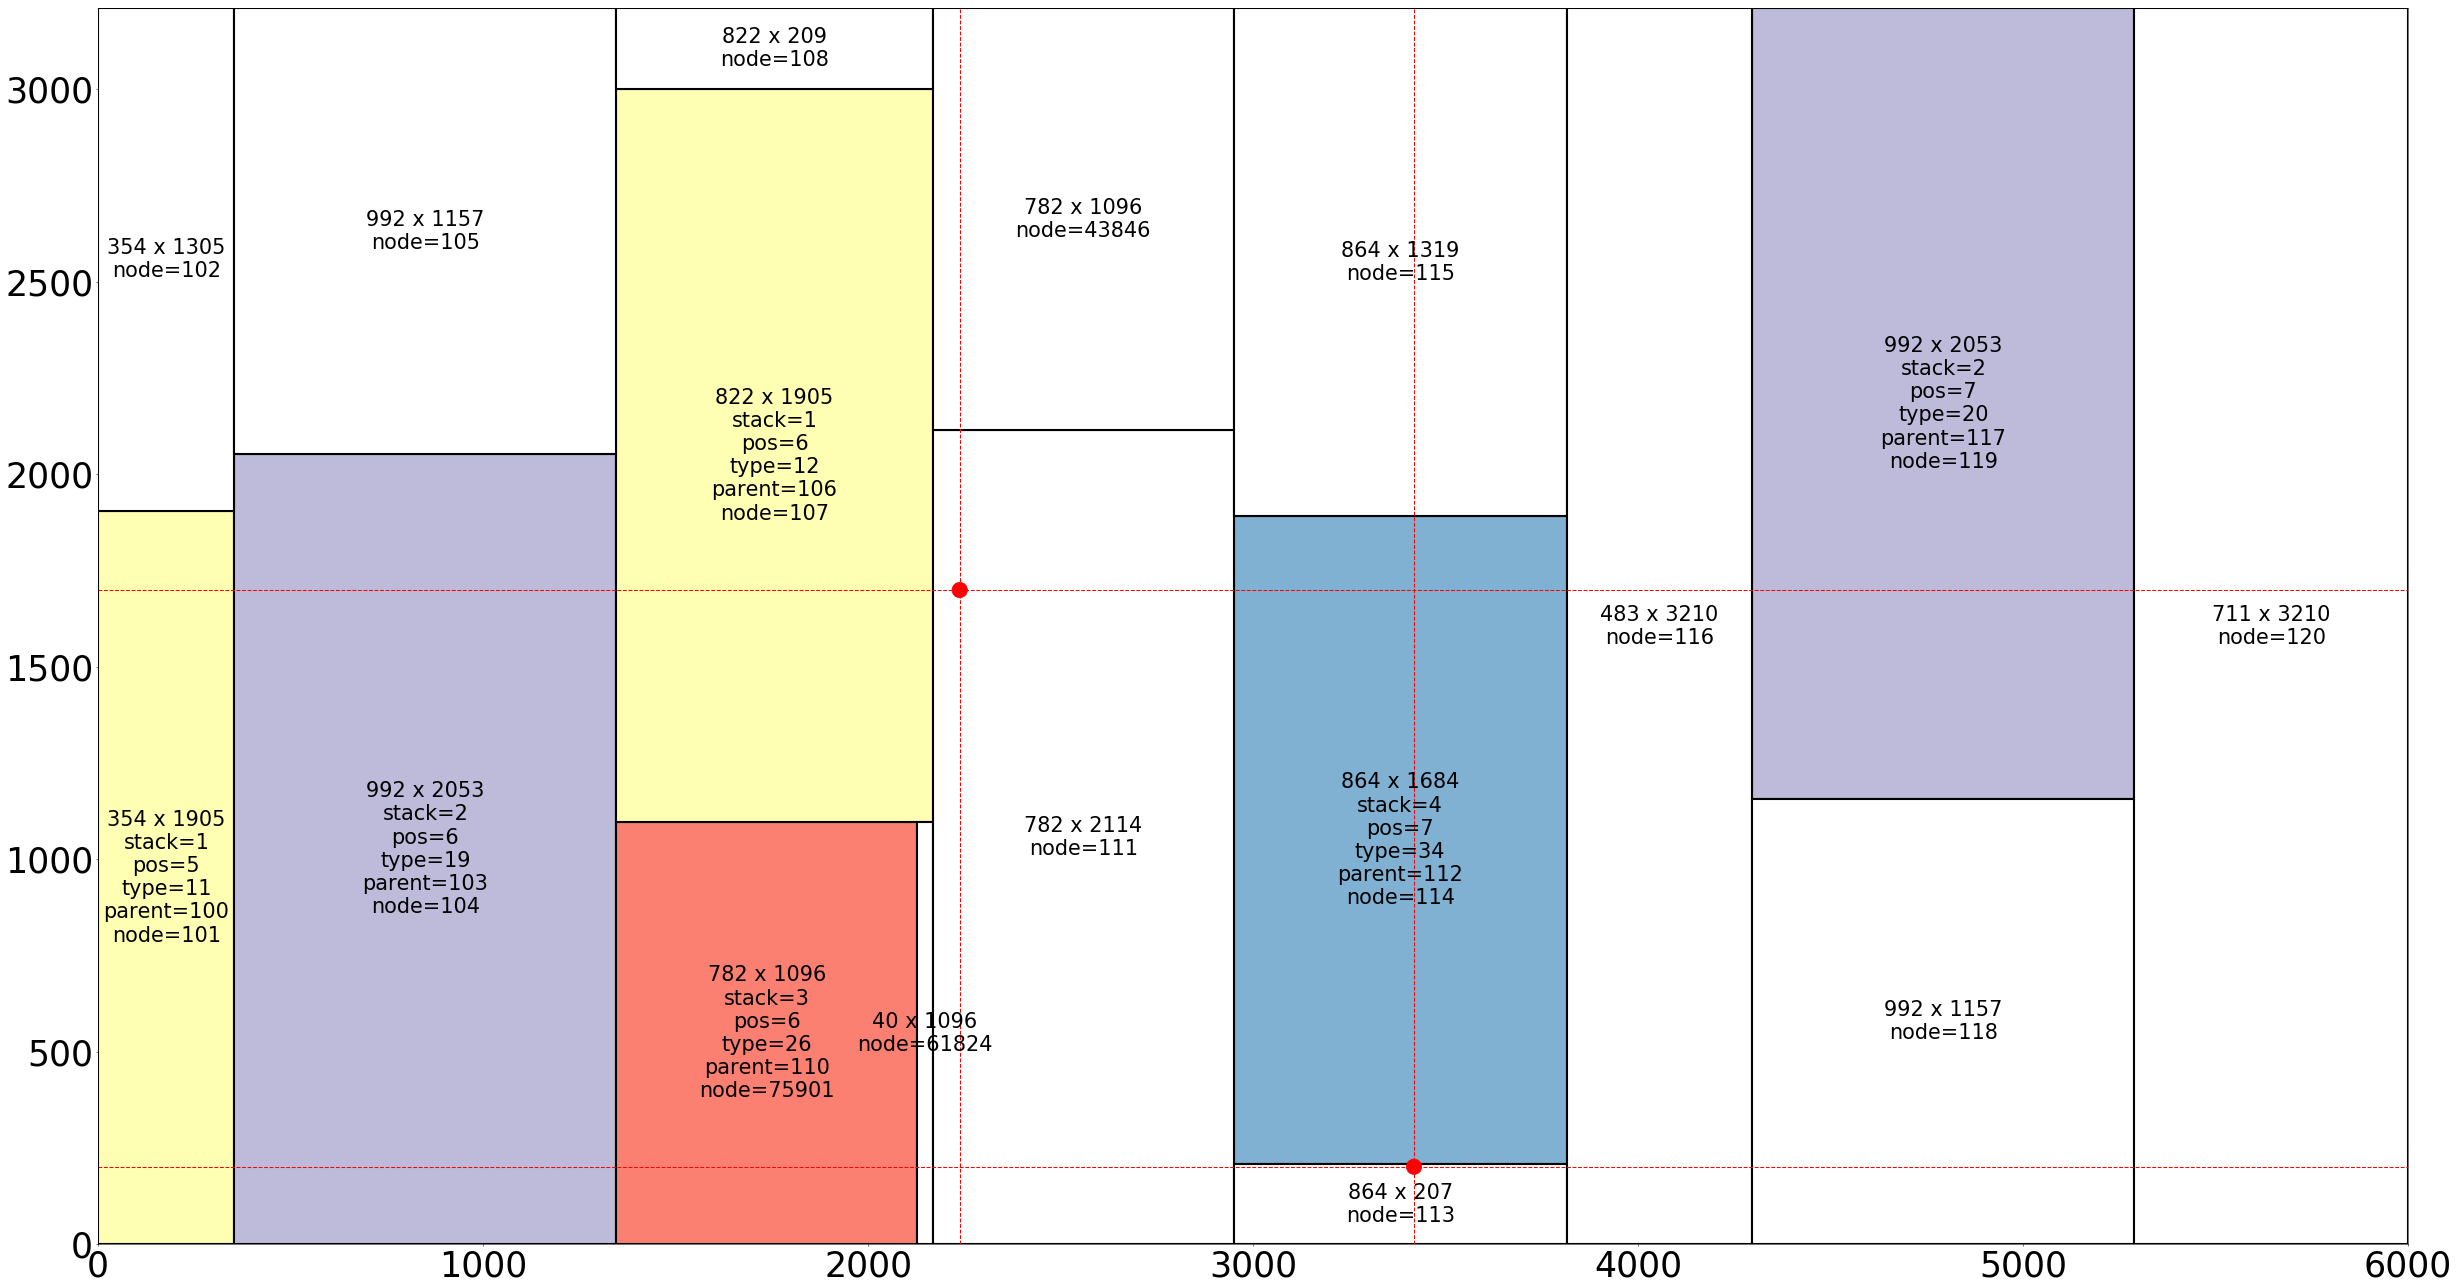
\includegraphics[width=0.7\linewidth]{swap_2_after.png}
            \caption{After swap level 2} \label{fig:swap2-after}
        \end{figure}

    \subsection{Complex insert}

        Figures \ref{fig:swap3-before} and \ref{fig:swap3-after} show an insert from a level 3 node (node 88, red) just before a level 2 (node 74, yellow) node while rotating it before insertion.

        \begin{figure}
            \centering
            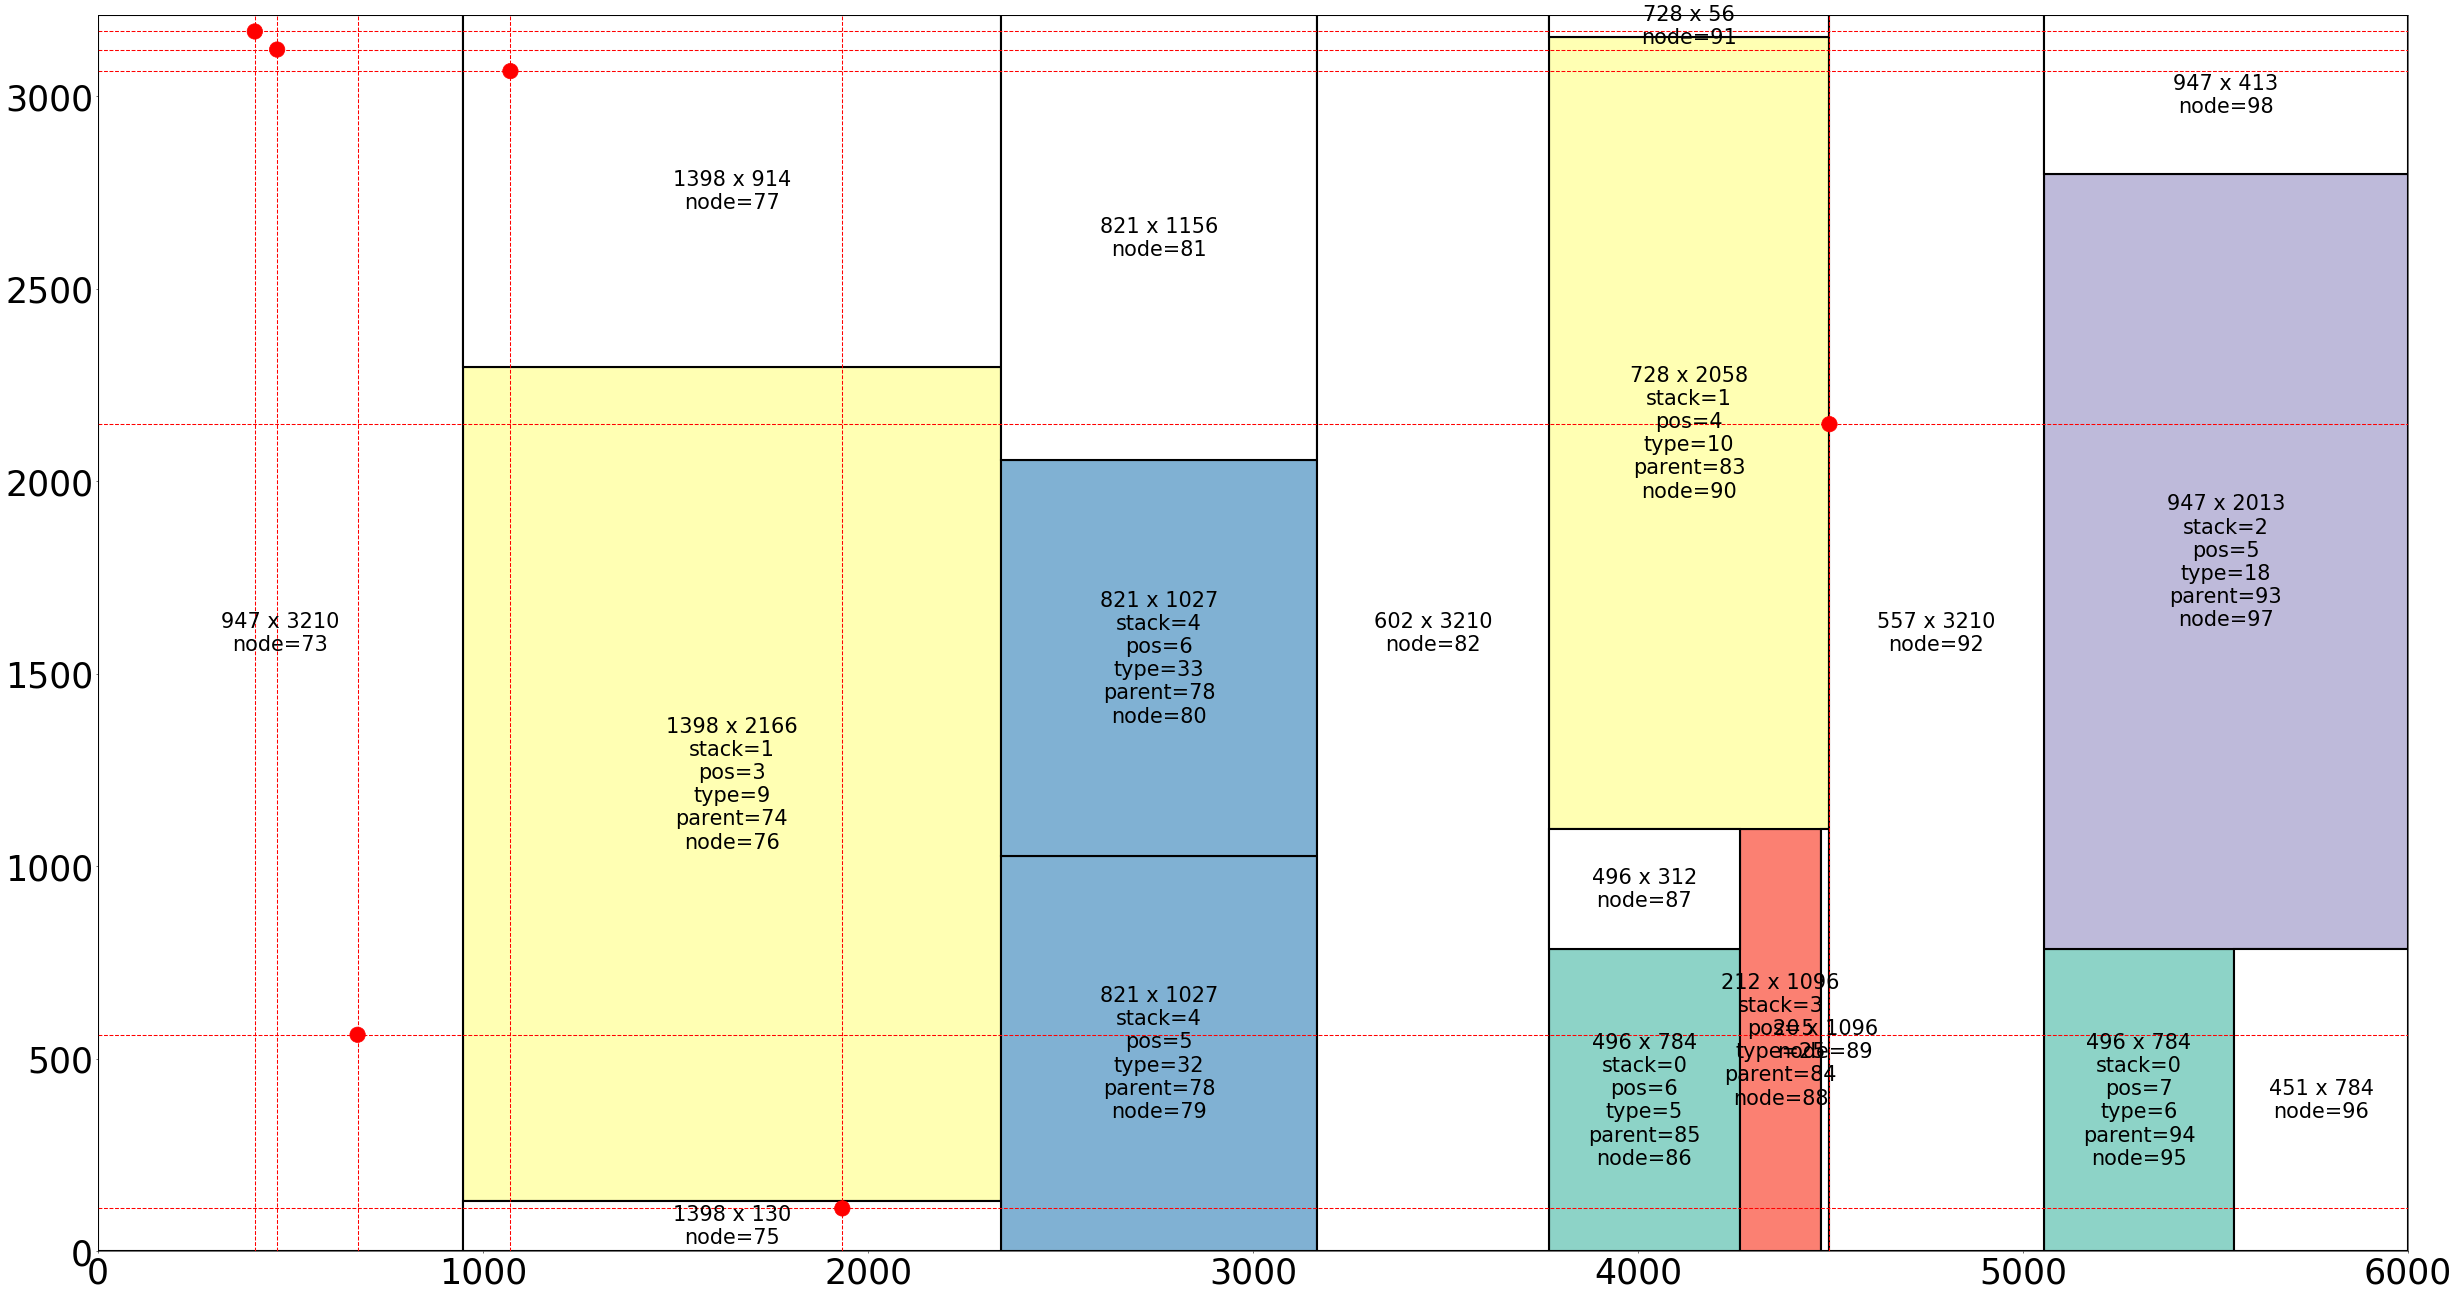
\includegraphics[width=0.7\linewidth]{swap_3_rot_before.png}
            \caption{before swap level 3} \label{fig:swap3-before}
        \end{figure}

        \begin{figure}
            \centering
            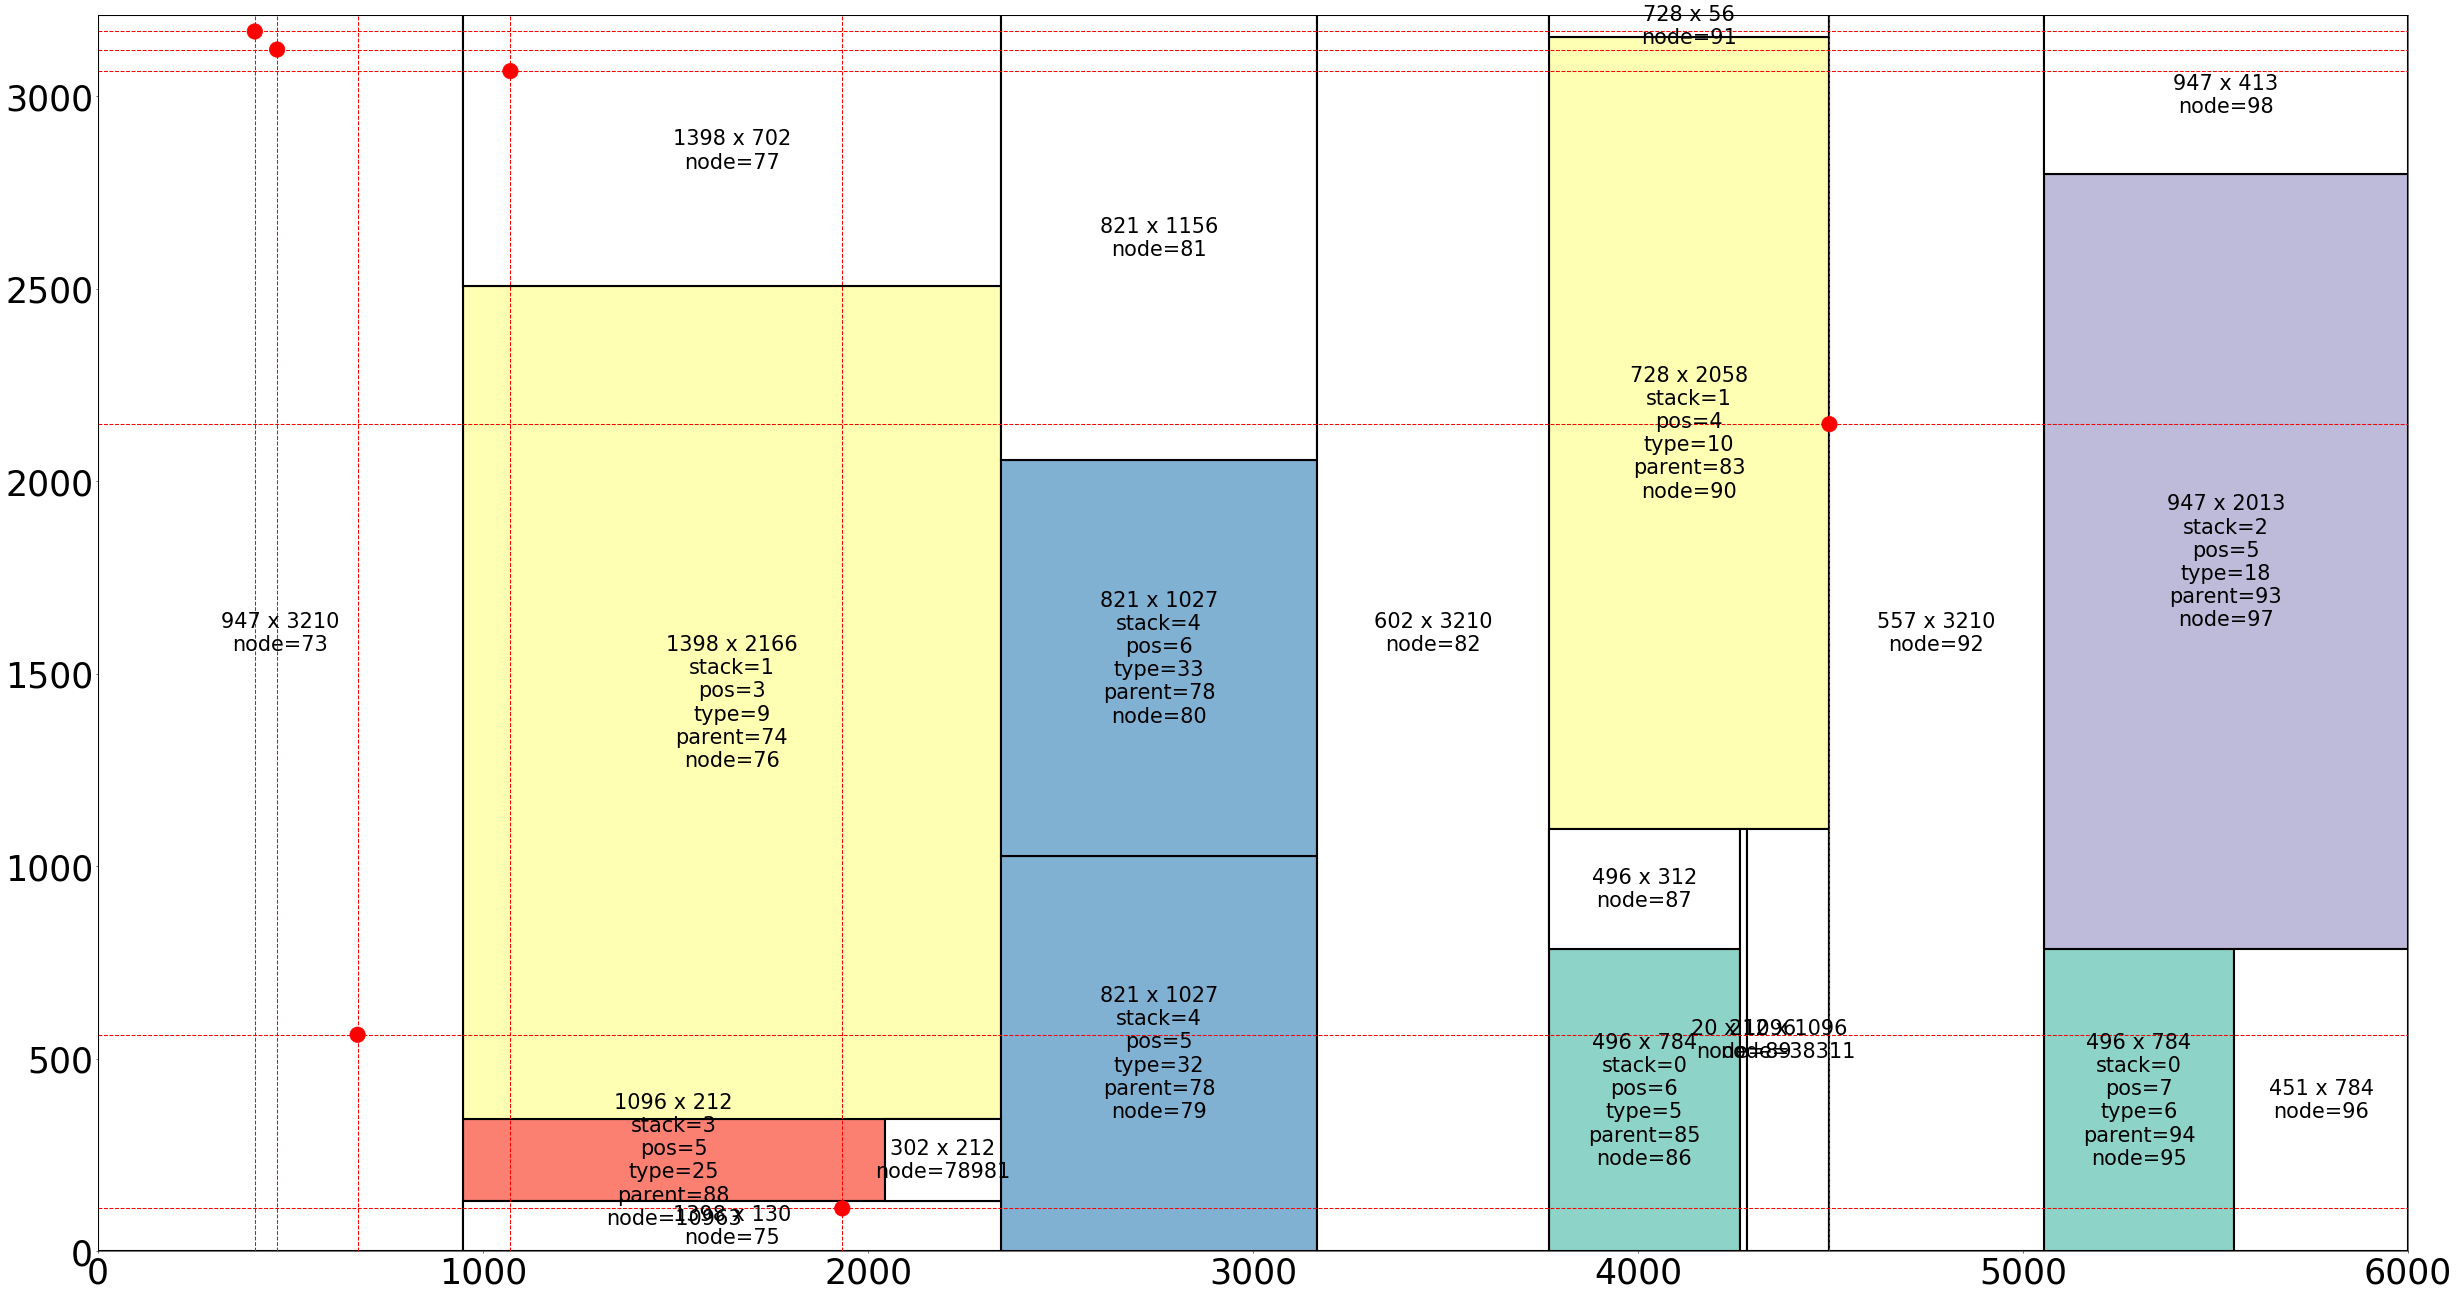
\includegraphics[width=0.7\linewidth]{swap_3_rot_after.png}
            \caption{After swap level 3} \label{fig:swap3-after}
        \end{figure}

        % ![before swap level 3\label{fig:}](.png)

        % ![After swap level 3\label{fig:swap3-after}](.png)

\section{Optimization}

    \subsection{Construction algorithm}

        An initial solution is done by ordering the nodes with many (random) feasible sequences and trying to insert them one after the other in the first available feasible whole in the jumbos. The best solution of all simulated is kept.

        This procedure to "create jumbos" is ran later with subsets of contiguous jumbos as part of an existing solution in order to try to find better neighbors.

    \subsection{Simulated annealing}

        The following changes are done at any of the three levels (between nodes of level 1, nodes of level 2 and nodes of level 3).

        \begin{enumerate}

            \item try to merge wastes that are neighbors into one single waste.
            \item create waste cuts following the positions of defects
            \item push wastes to the right of the solution (to the end).
            \item do swapping in same level to correct sequence.
            \item do swapping in same level to correct defects.
            \item do swapping in the same level from random pairs of nodes.
            \item make inter-level swaps of 1 level difference (1 and 2, 2 and 3, 3 and 4).
            \item make inter-level swaps of 2 level difference (1 and 3, 2 and 4).
            \item if not many changes, remake solution by:

            \begin{enumerate}
                \item reordering a sequence of jumbos of size 1-4, 
                \item restarting to another initial solution,
                \item restarting to the best solution found.
            \end{enumerate}

        \end{enumerate}

\section{Implementation} 

    All the code is built in the python programming language (tested with versions 3.5 and 3.6). For the tree support, the following library was used: https://pypi.python.org/pypi/ete3

    In addition to trying the `CPython` implementation, tests have been made with the `pypy` JIT implementation and using the cython compiler. It appears to be faster in some cases.
    
    The deployment depends on which version of python is being used but it's not so different one from the other. It usually just implies getting the good distribution of python, creating a virtual environment, installing the necessary packages with pip, modifying the parameters file, and running the code via the command line.

    For more details, there is a requirements file and a README with instructions on how to get all the necessary files to use the code.

    The creation of initial solutions and the remaking of existing ones is done by spawning parallel processes.

\section{Conclusions and future work} 

\bibliographystyle{plain}
% \selectlanguage{english}
% \bibliography{./../biblio/MFMP}

\end{document}
